\documentclass[11pt,letterpaper]{article}

\newenvironment{proof}{\noindent{\bf Proof:}}{\qed\bigskip}

\newtheorem{theorem}{Theorem}
\newtheorem{corollary}{Corollary}
\newtheorem{lemma}{Lemma} 
\newtheorem{claim}{Claim}
\newtheorem{fact}{Fact}
\newtheorem{definition}{Definition}
\newtheorem{assumption}{Assumption}
\newtheorem{observation}{Observation}
\newtheorem{example}{Example}
\newcommand{\qed}{\rule{7pt}{7pt}}

\newcommand{\solution}[4]{
\thispagestyle{plain} 
\newpage
\setcounter{page}{1}
\noindent
\begin{center}
\framebox{ \vbox{
\vspace{4mm}
\vspace{0.2in} 
{\centering \large\mbox{#3}}\\
\vspace{0.1in}
{#1 \hfill {Date: #2}}
}}
\end{center}
\markright{#1}
}

\newenvironment{algorithm}
{\begin{center}
\begin{tabular}{|l|}
\hline
\begin{minipage}{1in}
\begin{tabbing}
\quad\=\qquad\=\qquad\=\qquad\=\qquad\=\qquad\=\qquad\=\kill}
{\end{tabbing}
\end{minipage} \\
\hline
\end{tabular}
\end{center}}

\def\Comment#1{\textsf{\textsl{$\langle\!\langle$#1\/$\rangle\!\rangle$}}}



\usepackage{graphicx, amssymb, amsmath, listings, float, mathtools}
\usepackage{color, url}
\lstset{language = Python}
\lstset{breaklines}
\lstset{extendedchars=false}

\oddsidemargin 0in
\evensidemargin 0in
\textwidth 6.5in
\topmargin -0.6in
\textheight 9.0in

\begin{document}

\solution{\large Jifu Zhao}{\large 10/21/2016}{\bf \Large ECE 544NA \hspace{0.5cm} 
		Fall 2016 \hspace{0.5cm} Assignment 3}

\section*{\Large I. Pencil-and-Paper}
\begin{description}
%%%%%%%%%%%%%%%%%%%%%%%%%%%%%%%%%%%%%%%%%%%%%%%%%%%%%%%%%%%%%%%%%%%%%%%%%%%%%%%%%%%%%%%%%
% Problem 1
\item{\bf \large 1. E-Step}

Since that $p_{X|\Theta(x_i|\theta)}$ is described as:
\begin{equation}
	p_{X|\Theta(x_i|\theta)} = \sum_{h=1}^{m} w_h p_{V|H, \Theta}(x_i, h, \theta)
\end{equation}

The corresponding log-likelihood is:
\begin{equation}
\begin{split}
log\mathcal{L}(\Theta) = \sum_{i=1}^n log(\sum_{h=1}^m w_h p_{V|H, \Theta}(x_i, h, \theta))
\end{split} 
\end{equation}

Now, suppose the hidden variable is $y$, where $y$ could be 1, 2, $\cdots$, m. Then, we can calculate the expectation of the log-likelihood $E[log\mathcal{L}(\Theta)]$ as:
\begin{equation}
\begin{split}
E[log\mathcal{L}(\Theta)] = \sum_{k=1}^m [\sum_{i=1}^n log(\sum_{h=1}^m w_h p_{V|H, \Theta}(x_i, h, \theta | y=k))] \cdot \gamma_i(k)
\end{split} 
\end{equation}
where $\gamma_i(k)$ is the posterior probability for $y = k$, and $\gamma_i(k)$ is defined as:
\begin{equation}
	\gamma_i(k) = \frac{w_k \mathcal{N}(x_i; \mu_k, \Sigma_k)}{\sum_l w_l \mathcal{N}(x_i; \mu_l, \Sigma_l)}
\end{equation}

Also, notice that 
\begin{equation}
p_{V|H, \Theta}(x_i, h, \theta | y=k)) = 
	\begin{cases}
		\mathcal{N}(x_i; \mu_k, \Sigma_k)  & \quad \text{if } h = k \\
		0 & \quad \text{if } h \neq k
	\end{cases}
\end{equation}

So, 
\begin{equation}
\begin{split}
E[log\mathcal{L}(\Theta)] & = \sum_{i=1}^n \sum_{k=1}^m log(w_k p_{V|H, \Theta}(x_i, h=k, \theta)) \cdot \gamma_i(k) \\
						  & =  \sum_{i=1}^n \sum_{k=1}^m log(w_k \mathcal{N}(x_i; \mu_k, \Sigma_k))\cdot \frac{w_k \mathcal{N}(x_i; \mu_k, \Sigma_k)}{\sum_l w_l \mathcal{N}(x_i; \mu_l, \Sigma_l)} \\
						  & = \sum_{i=1}^n \sum_{k=1}^m log(w_k \mathcal{N}(x_i; \mu_k, \Sigma_k))\cdot \gamma_i(k)
\end{split} 
\end{equation}

So, in E-Step, the most important thing is to calculate $\gamma_i(k)$ for each i and k, where 
\begin{equation}
\gamma_i(k) = \frac{w_k \mathcal{N}(x_i; \mu_k, \Sigma_k)}{\sum_l w_l \mathcal{N}(x_i; \mu_l, \Sigma_l)}
\end{equation}
And $\mathcal{N}(x_i; \mu_l, \Sigma_l)$ is defined as:
\begin{equation}
	\mathcal{N}(x_i; \mu_l, \Sigma_l) = \frac{1}{det(2 \pi \Sigma_l)}exp(-\frac{1}{2}(x_i - \mu_l)^T \Sigma_l^{-1} (x_i - \mu_l))
\end{equation}


%%%%%%%%%%%%%%%%%%%%%%%%%%%%%%%%%%%%%%%%%%%%%%%%%%%%%%%%%%%%%%%%%%%%%%%%%%%%%%%%%%%%%%%%%
% Problem 2
\item{\bf \large 2. M-Step}

From above equation (5), our goal is the maximize the expectation of log-likelihood $E[log\mathcal{L}(\Theta)]$.

First, consider $w_k$. With the constraint of $\sum_k w_k = 1$, we have:
\begin{equation}
\frac{\partial}{\partial w_k} [\sum_{i=1}^n \sum_{k=1}^m log(w_k \mathcal{N}(x_i; \mu_k, \Sigma_k))\cdot \gamma_i(k) + \lambda(\sum_k w_k - 1)] = 0
\end{equation}

So, we have: 
\begin{equation}
\sum_{i=1}^n \frac{\gamma_i(k)}{w_k} + \lambda = 0
\end{equation}

Summing it over k from 1 to m and with the equation that $\sum_k \gamma_i(k) = 1$, we can have:
\begin{equation}
\lambda = n
\end{equation}

So, we have:
\begin{equation}
	w_k^{new} = \frac{1}{n} \sum_{i=1}^n \gamma_i(k)
\end{equation}

Now, let's consider $\mu_k$ and $\Sigma_k$. Following the steps in {\it A gentle tutorial of the EM algorithm and its application to parameter estimation for Gaussian mixture and hidden Markov models}, we can simply get the following result:
\begin{equation}
	\mu_k^{new} = \frac{\sum_{i=1}^n x_i \gamma_i(k)}{\sum_{i=1}^n \gamma_i(k)}
\end{equation}


\begin{equation}
	\Sigma_k^{new} = \frac{\sum_{i=1}^n (x_i - \mu_k^{new}) \cdot (x_i - \mu_k^{new})^T \cdot \gamma_i(k)}{\sum_{i=1}^n \gamma_i(k)}
\end{equation}

So, Equation (12), (13) and (14) are the main steps for M-Step.

Following Equation (7), (12), (13) and (14), we can iterate through E-Step and M-Step until reaching some stop criteria.

\end{description}

\newpage
\section*{\Large II. Code-from-Scratch}

\subsection*{\large 1. Methods}

(1). The overall structure of the EM part is shown in Figure \ref{fig:structure}, which is named EM.py.

\begin{figure}[H]
\centering
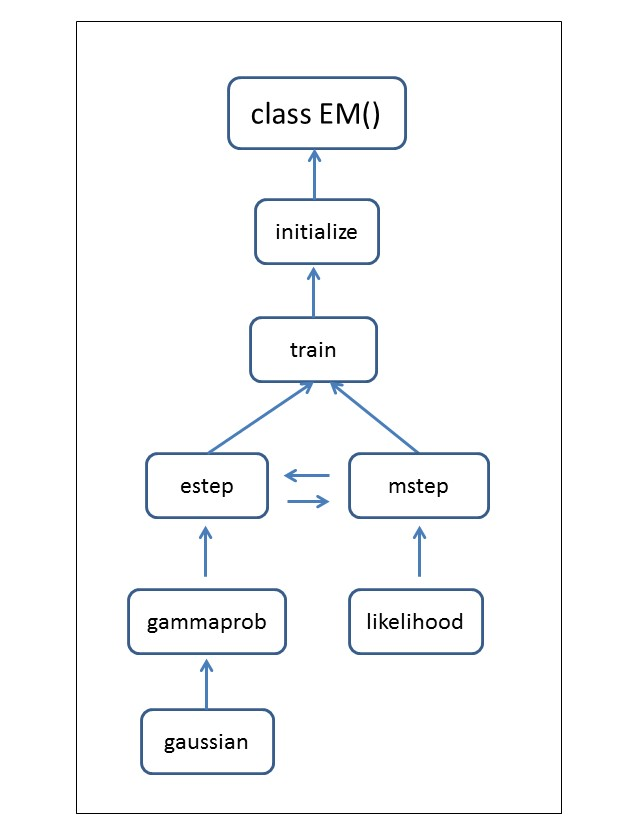
\includegraphics[width=0.7\textwidth]{./figures/ECE544hw3.jpg}
\caption{\label{fig:structure} Algorithm Structure}
\end{figure}

The whole program has initialize, train, estep, mstep, gammaprob, gaussian, likelihood part (get\_label and get\_params are not shown in this figure). These functions are based above each other.\\

(2). For the EM algorithm, the final goal is to determine m Gaussian mixtures that can best represent the original data.

Suppose that we are going to train a GMM model with m mixtures, and the original data has n samples and each has d features. Then, there are m weights, m means and each has d dimensions. Also, there are m covariance matrix, each of which has $d^2$ dimensions. So, the number of trainable parameters are:
$$ m + m d + m d^2 = m (1 + d + d^2)$$

\noindent {\bf *Note}: In our case, to avoid some computation problems, although the origin input image is in RGB format, whose range is from 0 to 255. In the following program, we first change the input image value range from [0, 255] to [0, 1].

\subsection*{\large 2. Results}

(1). In the first part, the original image is shown in Figure \ref{fig:corgi}.
\begin{figure}[H]
\centering
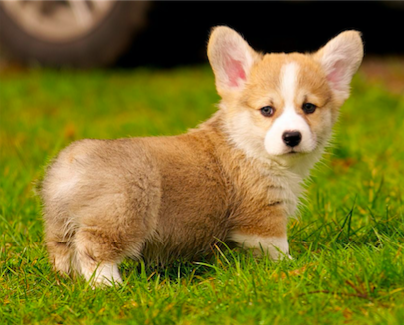
\includegraphics[width=0.6\textwidth]{./figures/corgi.png}
\caption{\label{fig:corgi} Original Dog Figure}
\end{figure}

First, choosing m = 3, we can get three Gaussian Mixture model, the corresponding weights, mean and covariance matrix is shown below:
$$ w_1 = 0.29569 $$
$$ w_2 = 0.31897 $$
$$ w_3 = 0.38534 $$
And the mean vector is:
$$ \vec{\mu_1} = [0.24586, \  0.22526, \  0.07403]^T$$
$$ \vec{\mu_2} = [0.76036, \  0.59326, \  0.41495]^T$$
$$ \vec{\mu_3} = [0.44742, \  0.50353, \  0.00079]^T$$
The corresponding covariance matrix is:
$$\Sigma_1 =
\begin{bmatrix}
	0.05137	&	0.04574	&	0.01579 \\ 
	0.04574	&	0.04544	&	0.01191 \\
	0.01579	&	0.01191	&	0.00864	\\
\end{bmatrix}$$

$$\Sigma_2 =
\begin{bmatrix}
	0.02177	&	0.02319	&	0.02469 \\ 
	0.02319	&	0.02691	&	0.03041 \\
	0.02469	&	0.03041	&	0.03740	\\
\end{bmatrix}$$

$$\Sigma_3 =
\begin{bmatrix}
	0.00741	&	0.00399	&	0.00002 \\ 
	0.00399	&	0.00441	&	0.00000 \\
	0.00002	&	0.00000	&	0.00001	\\
\end{bmatrix}$$


\noindent {\bf *Note}: During the training process, we notice that the initialization has a big effect on the final output. In other words, we have chances to reach some local maximum rather than the global maximum. So, every time we run the code, we could get total different result. A good initialization is to find some good points using K-means method, however, in this work, this method is not implemented.\\

(2). Choosing m to be 3, 5 and 10, through some fixed random initialization, we can reconstruct the original image. The result is shown in Figure \ref{fig:corgi_3}, Figure \ref{fig:corgi_5} and Figure \ref{fig:corgi_10}.

\begin{figure}[H]
\centering
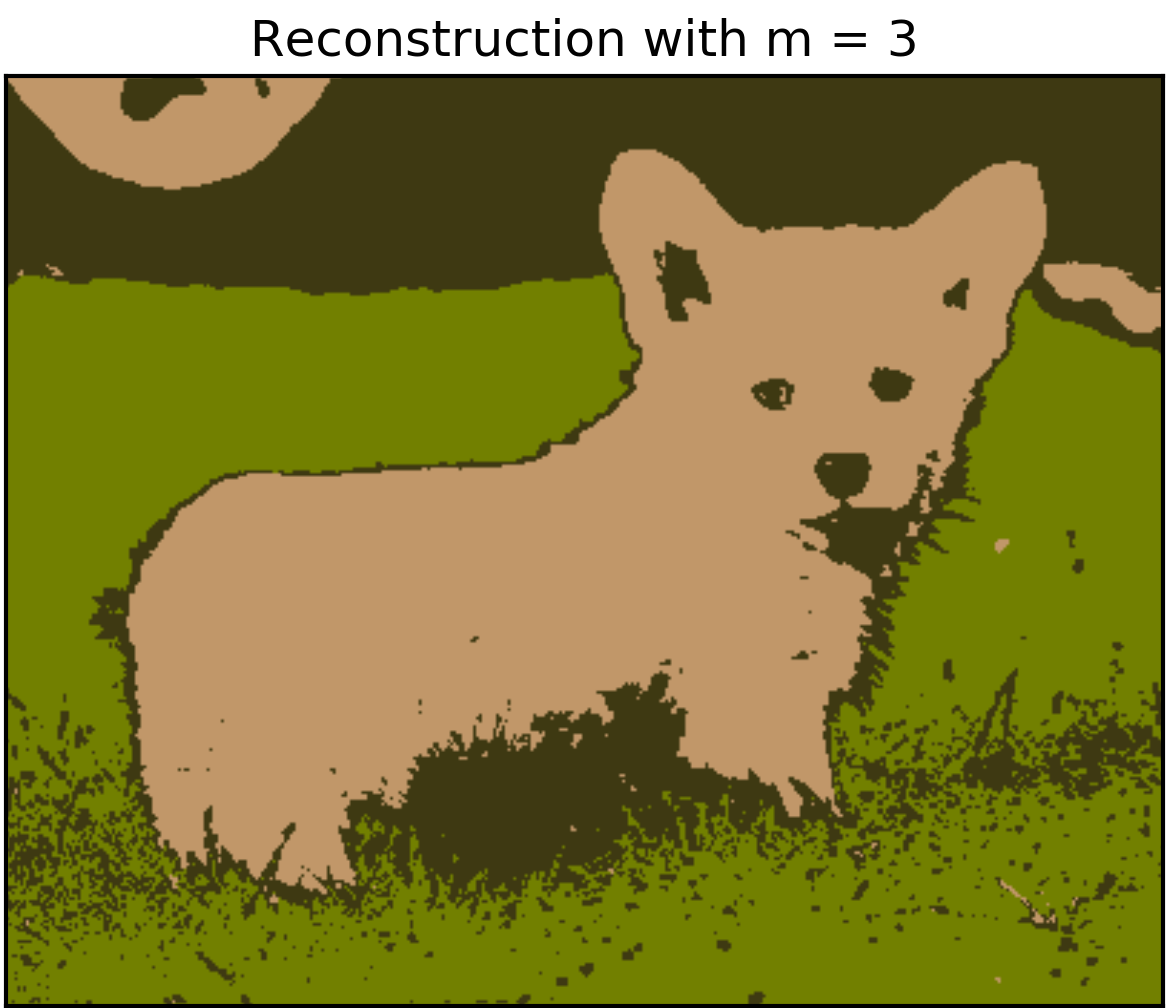
\includegraphics[width=0.6\textwidth]{./figures/corgi_3.png}
\caption{\label{fig:corgi_3} Dog with 3 Gaussian Mixtures}
\end{figure}

\begin{figure}[H]
\centering
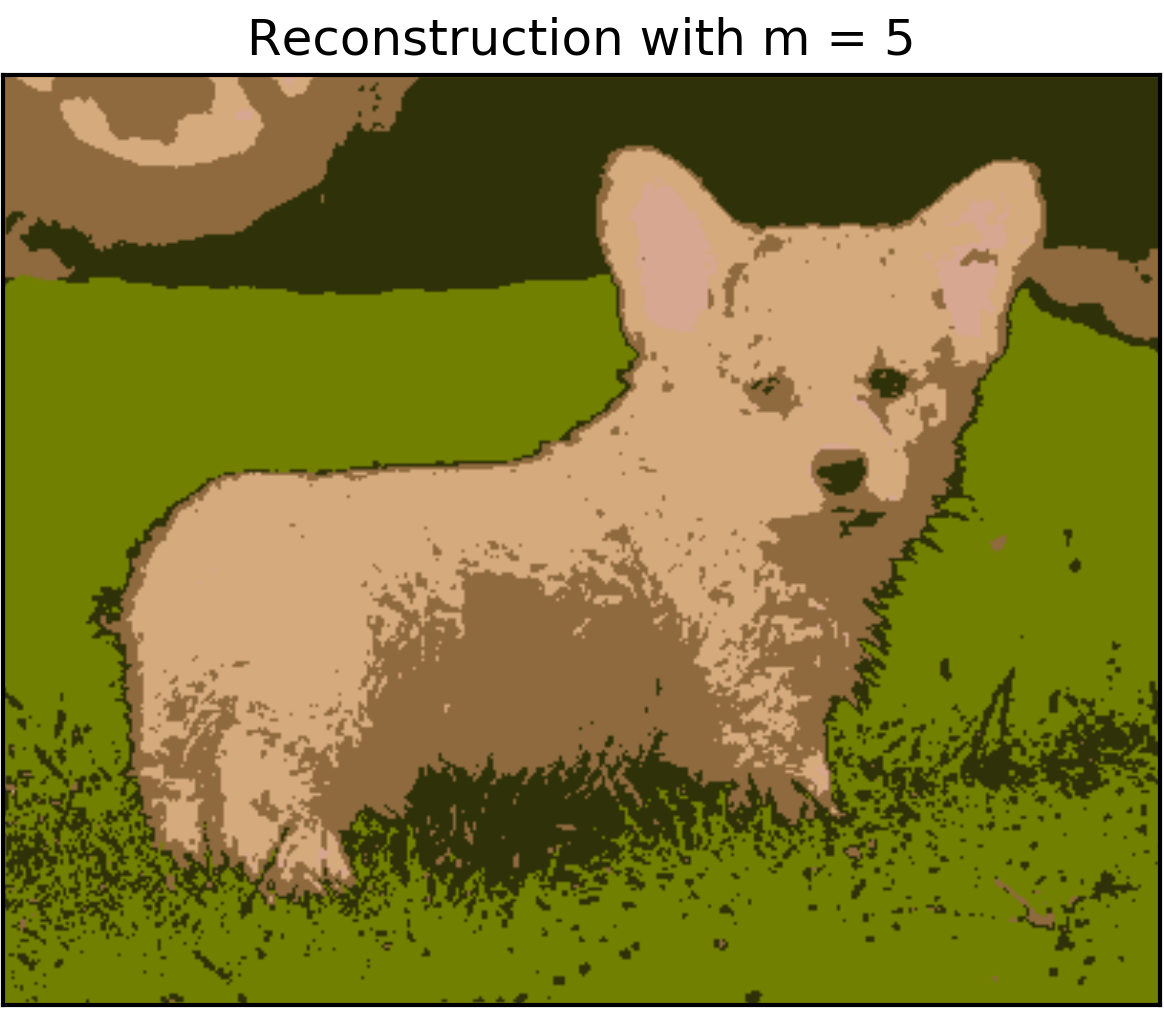
\includegraphics[width=0.6\textwidth]{./figures/corgi_5.png}
\caption{\label{fig:corgi_5} Dog with 5 Gaussian Mixtures}
\end{figure}

\begin{figure}[H]
\centering
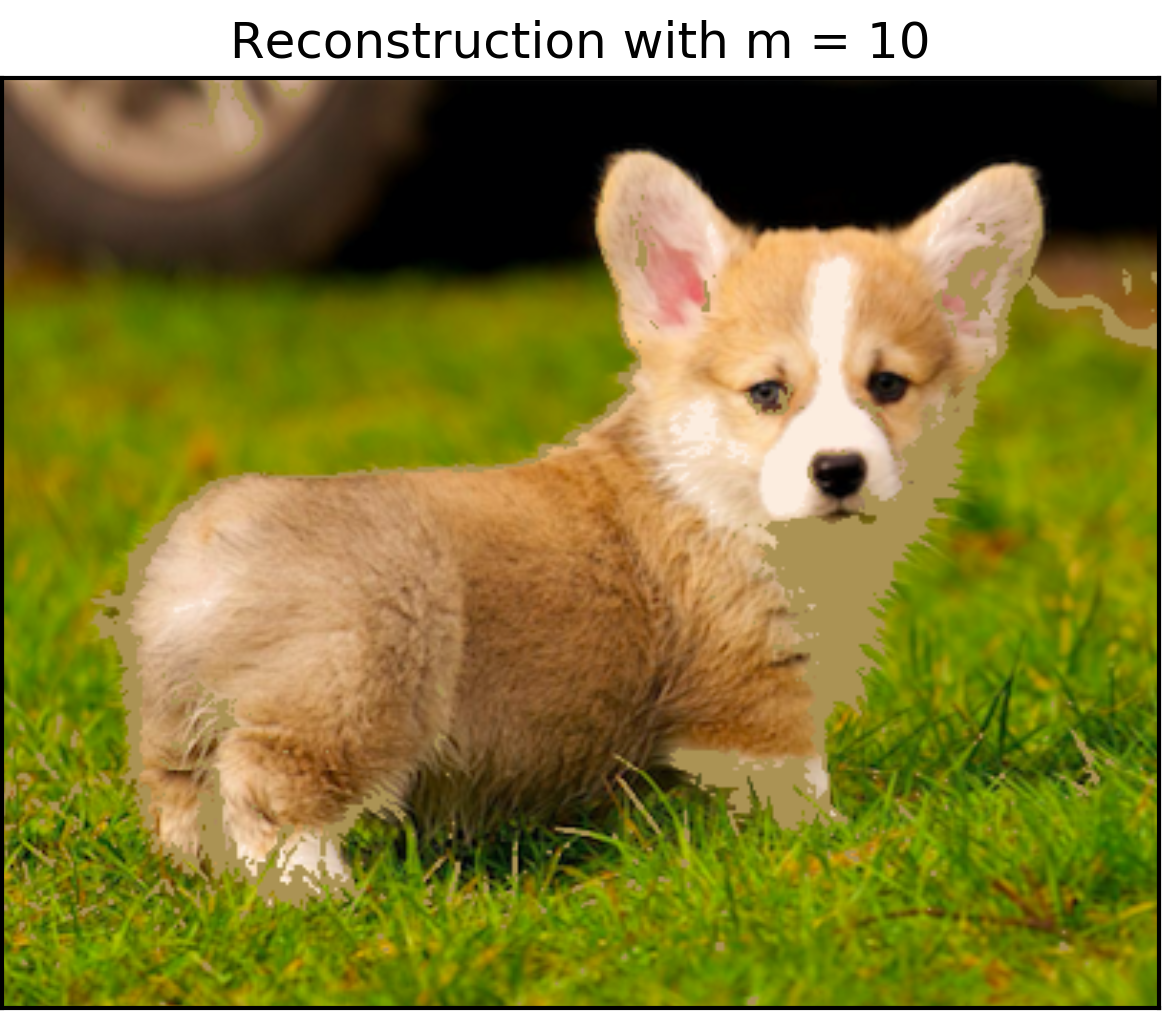
\includegraphics[width=0.6\textwidth]{./figures/corgi_10.png}
\caption{\label{fig:corgi_10} Dog with 10 Gaussian Mixtures}
\end{figure}

\newpage
(3). In this part, we choose one figure that contains mountains to test our model. The original image is shown in Figure \ref{fig:self}.
\begin{figure}[H]
\centering
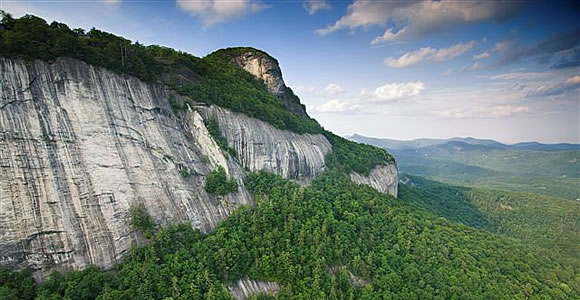
\includegraphics[width=0.6\textwidth]{./figures/self.jpg}
\caption{\label{fig:self} Original Mountain Figure}
\end{figure}

First, choosing m = 3, we can get three Gaussian Mixture model, the corresponding weights, mean and covariance matrix are shown below:
$$ w_1 = 0.19563 $$
$$ w_2 = 0.43580 $$
$$ w_3 = 0.36857 $$
And the mean vector is:
$$ \vec{\mu_1} = [0.49253, \  0.58691, \  0.72089]^T$$
$$ \vec{\mu_2} = [0.25903, \  0.35042, \  0.24338]^T$$
$$ \vec{\mu_3} = [0.61135, \  0.61422, \  0.61133]^T$$
The corresponding covariance matrix is:
$$\Sigma_1 =
\begin{bmatrix}
	0.03400	&	0.02849	&	0.02296 \\ 
	0.02849	&	0.02511	&	0.02183 \\
	0.02296	&	0.02183	&	0.02151	\\
\end{bmatrix}$$

$$\Sigma_2 =
\begin{bmatrix}
	0.01594 &	0.01579  &	0.01530 \\
  	0.01579 &	0.01677  &	0.01532 \\
  	0.01530 &	0.01532  &	0.01949 \\

\end{bmatrix}$$

$$\Sigma_3 =
\begin{bmatrix}
	0.04029  &	0.03880 &	0.03899 \\
  	0.03880  &	0.03778 &	0.03822 \\
  	0.03899  &	0.03822 &	0.03962 \\
\end{bmatrix}$$

Now, choosing m to be 3, 5 and 10, through some fixed random initialization, we can reconstruct the original image. The result is shown in Figure \ref{fig:self_3}, Figure \ref{fig:self_5} and Figure \ref{fig:self_10}.

\begin{figure}[H]
\centering
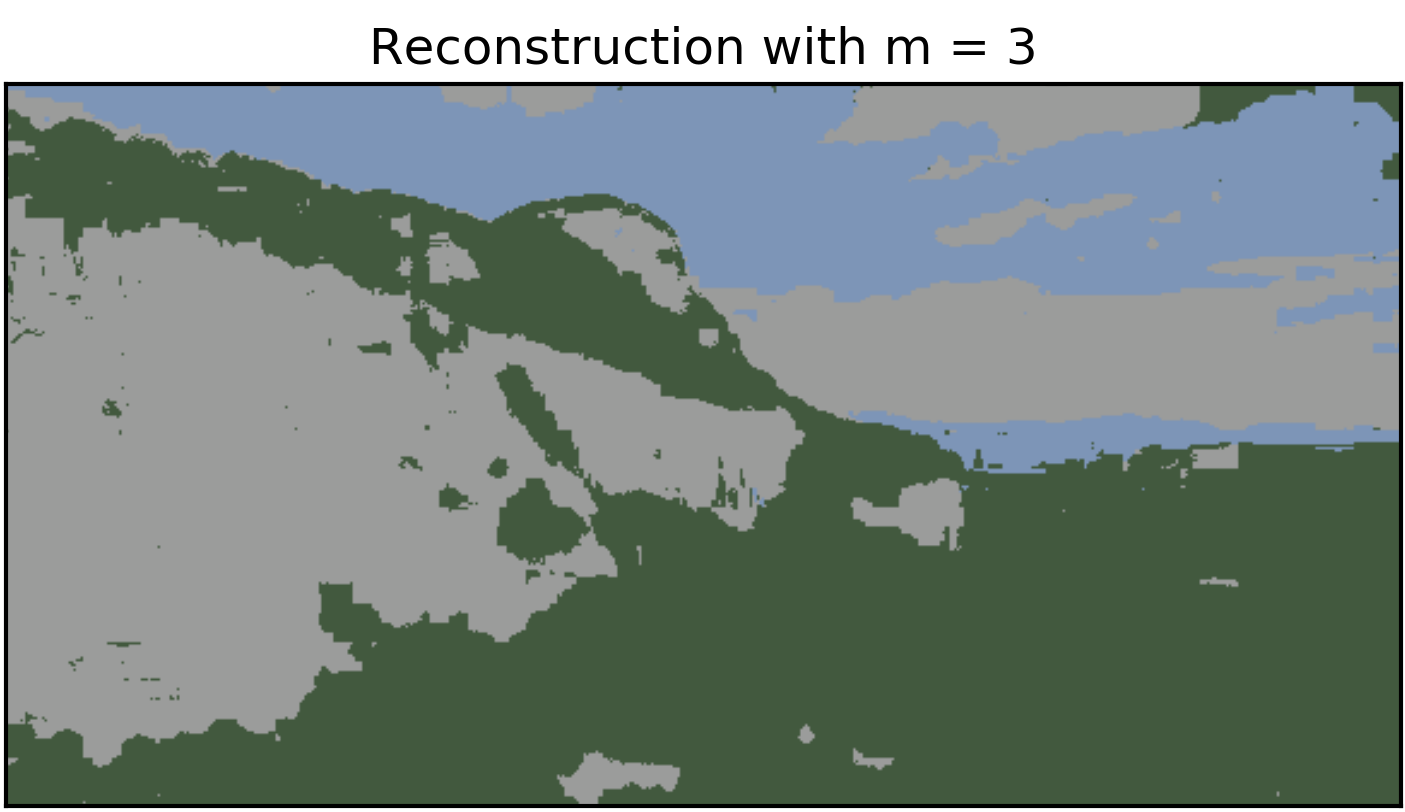
\includegraphics[width=0.6\textwidth]{./figures/self_3.png}
\caption{\label{fig:self_3} Mountain with 3 Gaussian Mixtures}
\end{figure}

\begin{figure}[H]
\centering
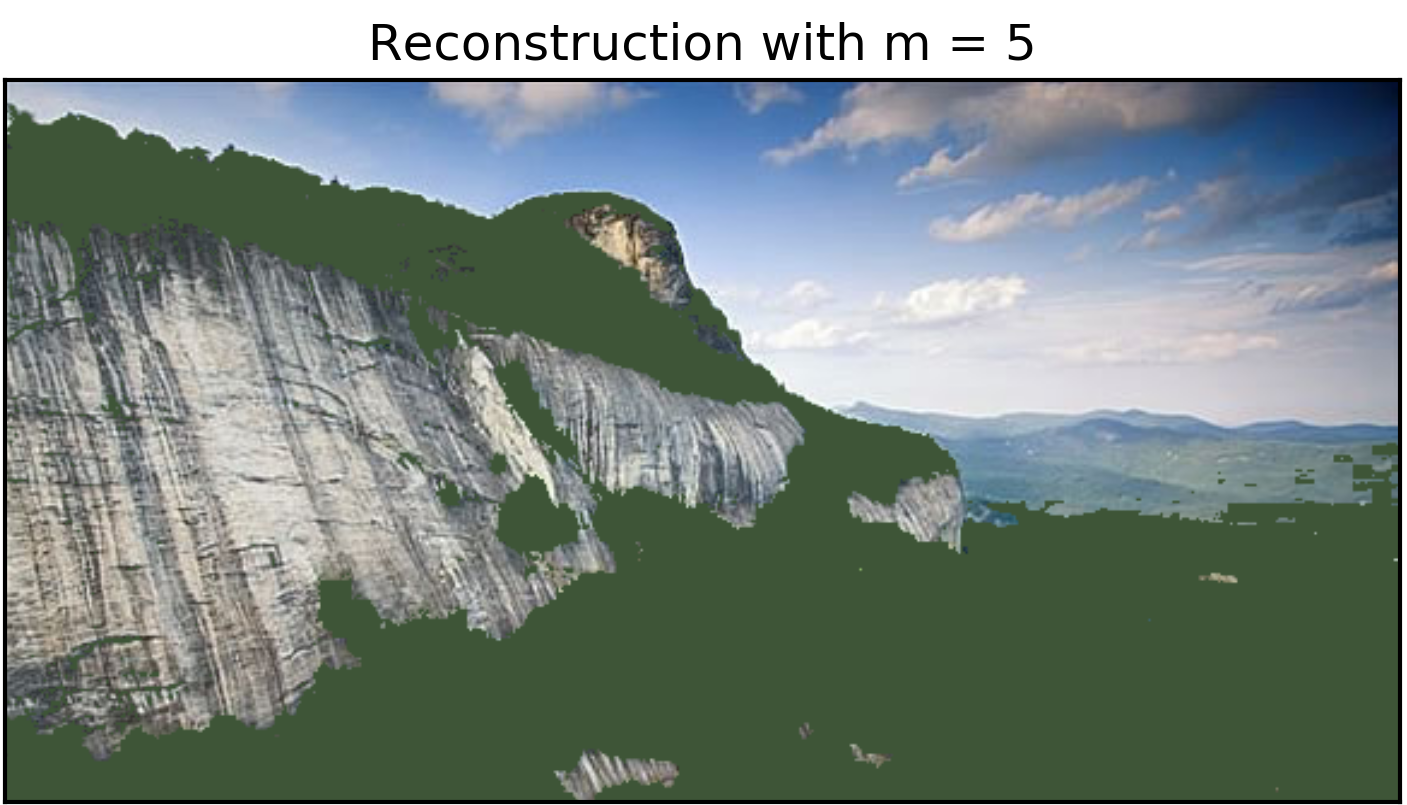
\includegraphics[width=0.6\textwidth]{./figures/self_5.png}
\caption{\label{fig:self_5} Mountain with 5 Gaussian Mixtures}
\end{figure}

\begin{figure}[H]
\centering
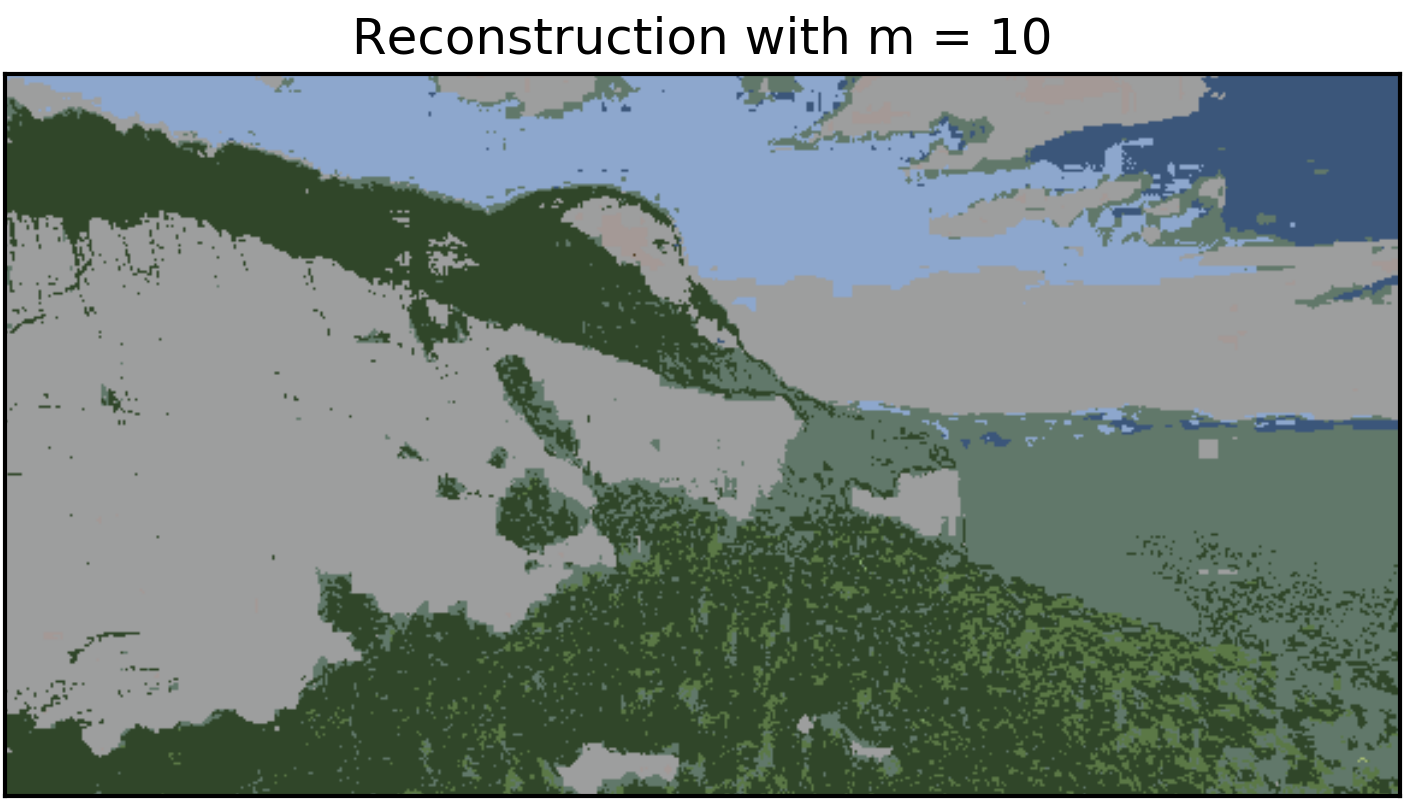
\includegraphics[width=0.6\textwidth]{./figures/self_10.png}
\caption{\label{fig:self_10} Mountain with 10 Gaussian Mixtures}
\end{figure}

\newpage
\section*{\Large III. TensorFlow}

\subsection*{\large 1. Methods}
In this section, we implemented the higher-level API from TenforFlow GMM. Since the original has already finished, we just simply import the module and build the GMM model through setting some parameters, such as num\_clusters, random\_seed, initial\_clusters, covariance\_type. In this part, we set the initial\_clusters to be random and set covariance\_type to be full. 
$$gmm = GMM(*args)$$
Then, we can fit our data through $$gmm.fit(x)$$
and then we can get the label through the function $$gmm.predict(x)$$

\subsection*{\large 2. Results}

(1). In the first part, the original image is Figure \ref{fig:corgi}, but we apply the GMM model from TensorFlow instead of our own model.

First, choosing m = 3, we can get three Gaussian Mixture model, the corresponding weights, mean and covariance matrix is shown below:
$$ w_1 = 0.26408 $$
$$ w_2 = 0.23359 $$
$$ w_3 = 0.50233 $$
And the mean vector is:
$$ \vec{\mu_1} = [0.76676, \  0.59889, \  0.42117]^T$$
$$ \vec{\mu_2} = [0.19277, \  0.16881, \  0.05494]^T$$
$$ \vec{\mu_3} = [0.45933, \   0.51962, \  0.00615]^T$$
The corresponding covariance matrix is:
$$\Sigma_1 =
\begin{bmatrix}
	0.01856 &	0.01889 &	0.02230 \\
  	0.01889 &	0.02332 &	0.02685 \\
  	0.02230 &	0.02685 &	0.03730 \\
\end{bmatrix}$$

$$\Sigma_2 =
\begin{bmatrix}
	0.03293 &	0.02596 &	0.00883	\\
  	0.02596 &	0.02639 &	0.00610	\\
  	0.00883 &	0.00610 &	0.00556 \\
\end{bmatrix}$$

$$\Sigma_3 =
\begin{bmatrix}
	0.01044 &	0.00437 &	0.00023 \\
  	0.00437 &	0.00520 &	0.00012 \\
  	0.00023 &	0.00012 &	0.00132 \\
\end{bmatrix}$$

(2). Choosing m to be 3, 5 and 10, through some fixed random initialization, we can reconstruct the original image. The result is shown in Figure \ref{fig:corgi_tf_3}, Figure \ref{fig:corgi_tf_5} and Figure \ref{fig:corgi_tf_10}.

\begin{figure}[H]
\centering
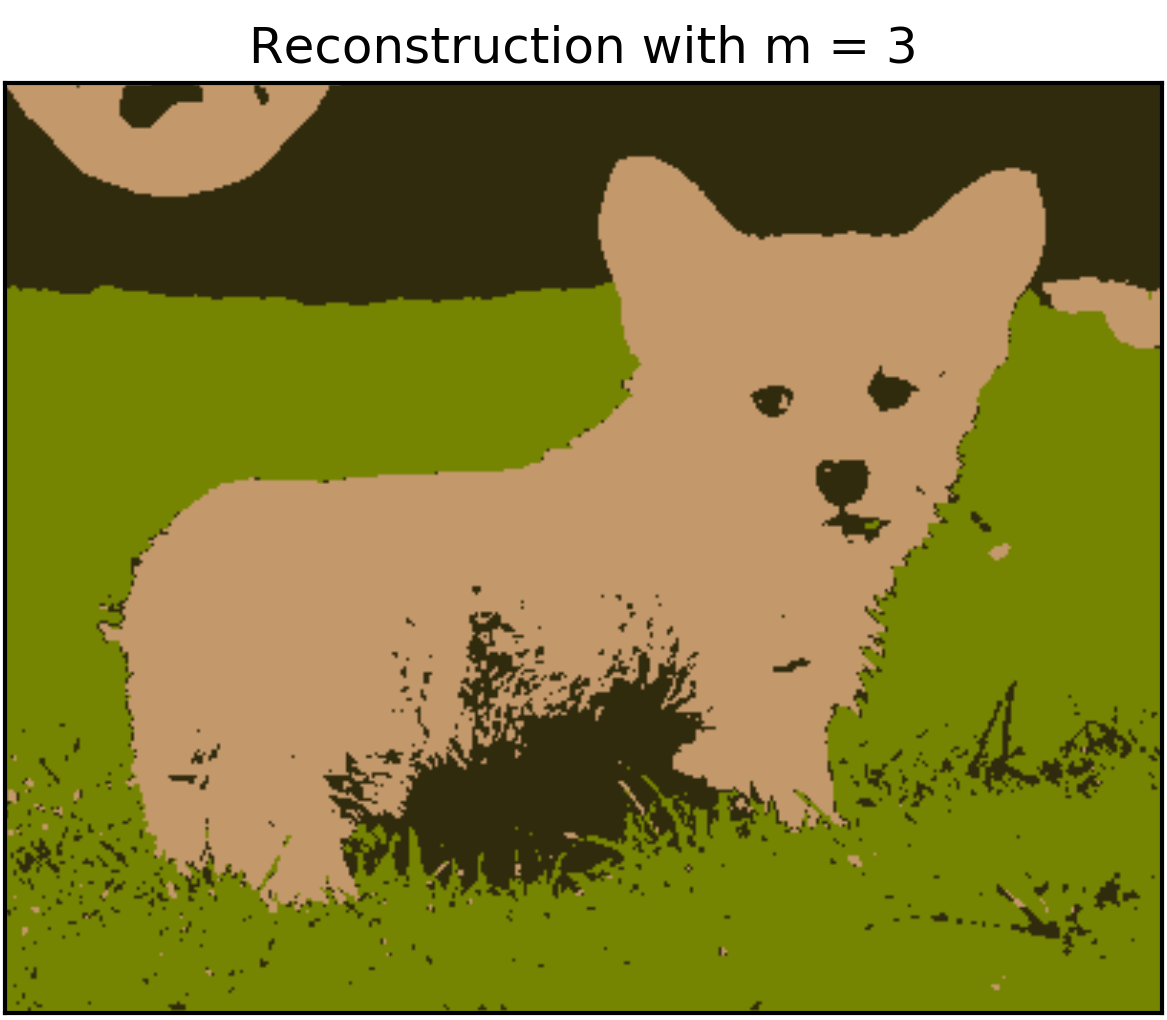
\includegraphics[width=0.6\textwidth]{./figures/corgi_tf_3.png}
\caption{\label{fig:corgi_tf_3} Dog with 3 Gaussian Mixtures}
\end{figure}

\begin{figure}[H]
\centering
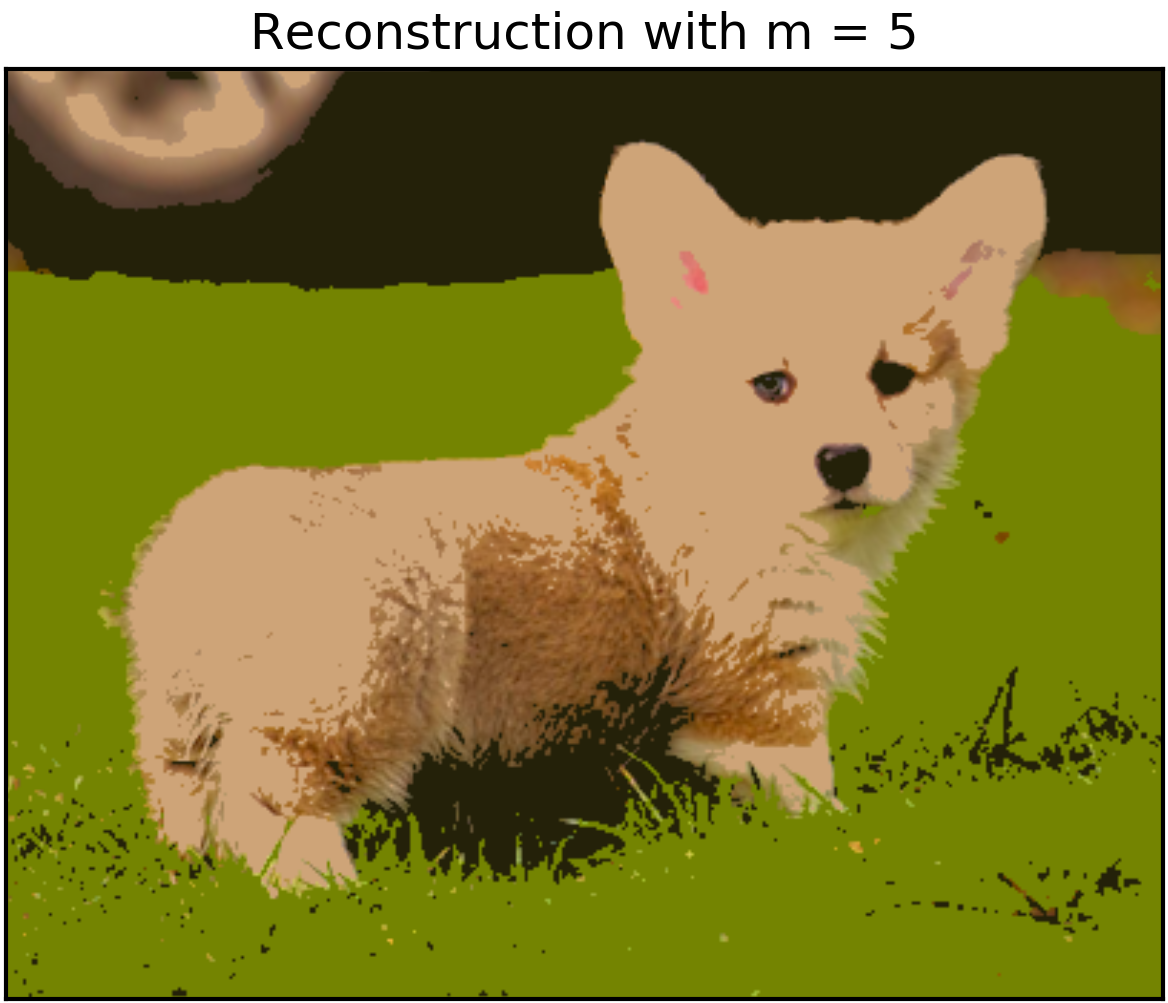
\includegraphics[width=0.6\textwidth]{./figures/corgi_tf_5.png}
\caption{\label{fig:corgi_tf_5} Dog with 5 Gaussian Mixtures}
\end{figure}

\begin{figure}[H]
\centering
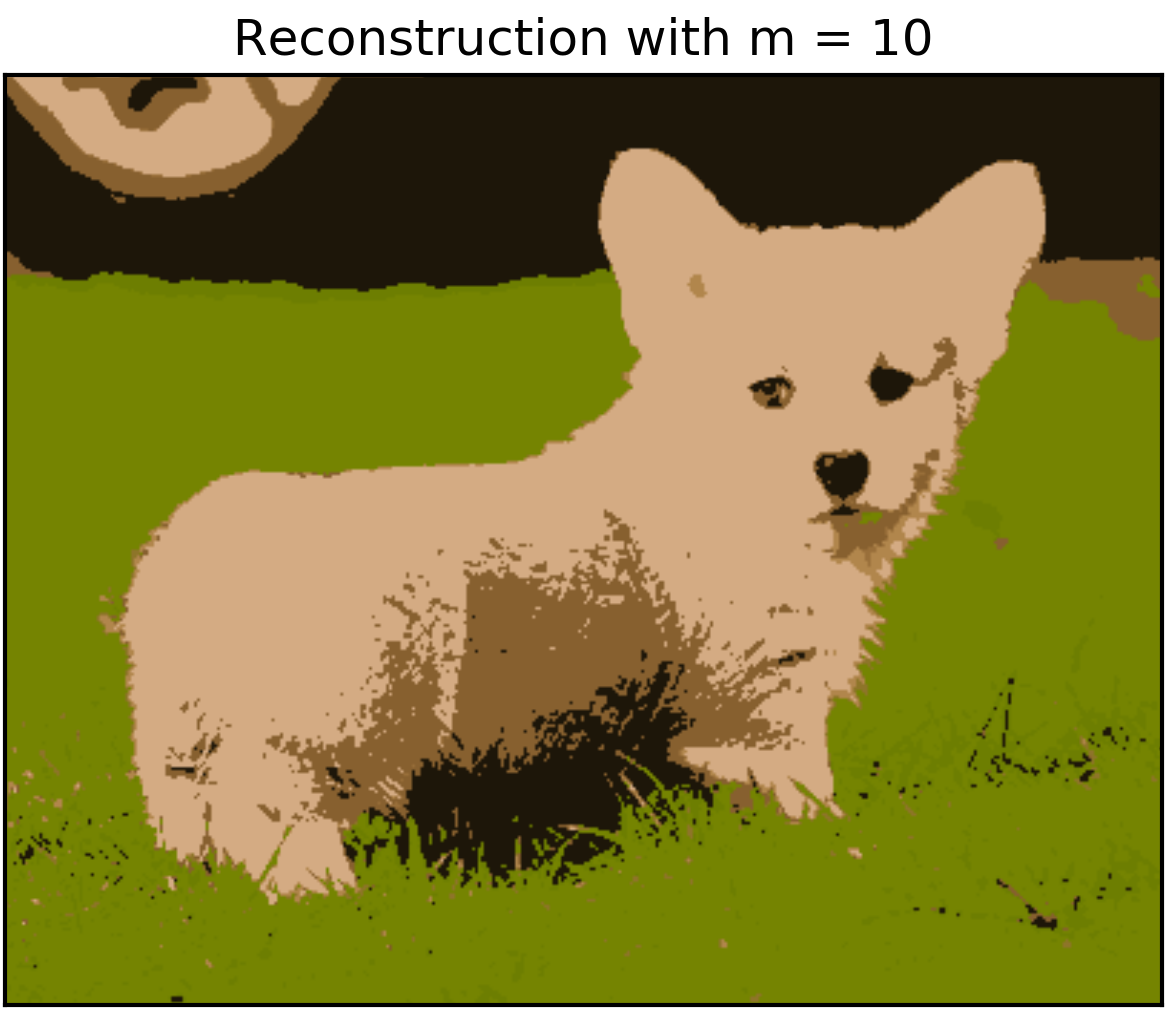
\includegraphics[width=0.6\textwidth]{./figures/corgi_tf_10.png}
\caption{\label{fig:corgi_tf_10} Dog with 10 Gaussian Mixtures}
\end{figure}

(3). In this part, we choose one figure that contains mountains to test our model. The original image is shown in Figure \ref{fig:self}, but we apply the GMM model from TensorFlow instead of our own model.

First, choosing m = 3, we can get three Gaussian Mixture model, the corresponding weights, mean and covariance matrix are shown below:
$$ w_1 = 0.36099 $$
$$ w_2 = 0.20816 $$
$$ w_3 = 0.43084 $$
And the mean vector is:
$$ \vec{\mu_1} = [0.70019, \  0.71285, \  0.72229]^T$$
$$ \vec{\mu_2} = [0.46636, \  0.54795, \  0.63692]^T$$
$$ \vec{\mu_3} = [0.23894, \  0.31741, \  0.23316]^T$$
The corresponding covariance matrix is:
$$\Sigma_1 =
\begin{bmatrix}
	0.02382 &	0.01941 &	0.01793 \\
  	0.01941 &	0.01833 &	0.01684 \\
  	0.01793 &	0.01684 &	0.02003 \\
\end{bmatrix}$$

$$\Sigma_2 =
\begin{bmatrix}
	0.02526 &	0.01735  &	0.00951 \\
  	0.01735 &	0.01567  &	0.01217 \\
  	0.00951 &	0.01217  &	0.02121 \\
\end{bmatrix}$$

$$\Sigma_3 =
\begin{bmatrix}
	0.01769 &	0.01662 &	0.01141 \\
  	0.01662 &	0.01926 &	0.01151 \\
  	0.01141 &	0.01151 &	0.01468 \\
\end{bmatrix}$$

Now, choosing m to be 3, 5 and 10, through some fixed random initialization, we can reconstruct the original image. The result is shown in Figure \ref{fig:self_tf_3}, Figure \ref{fig:self_tf_5} and Figure \ref{fig:self_tf_10}.

\begin{figure}[H]
\centering
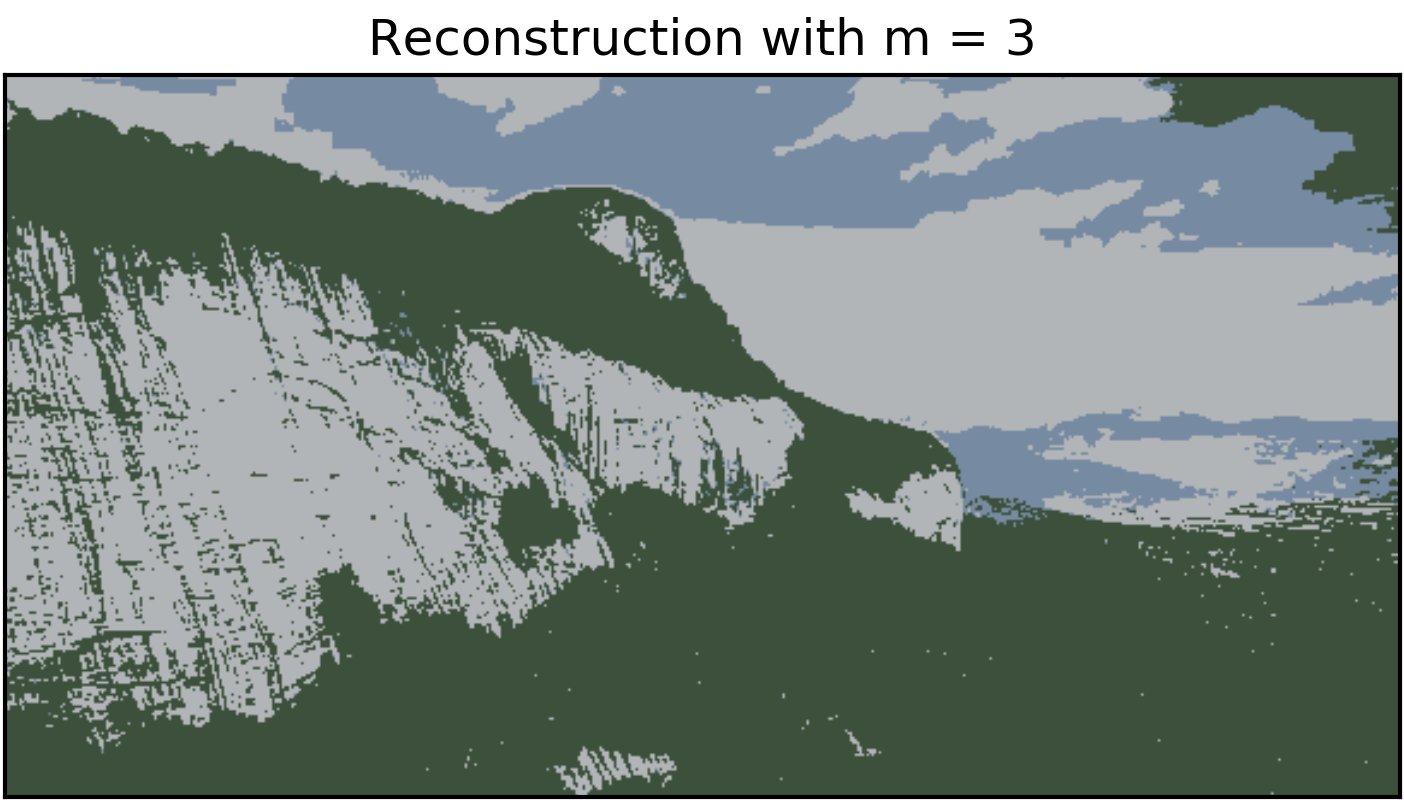
\includegraphics[width=0.6\textwidth]{./figures/self_tf_3.png}
\caption{\label{fig:self_tf_3} Mountain with 3 Gaussian Mixtures}
\end{figure}

\begin{figure}[H]
\centering
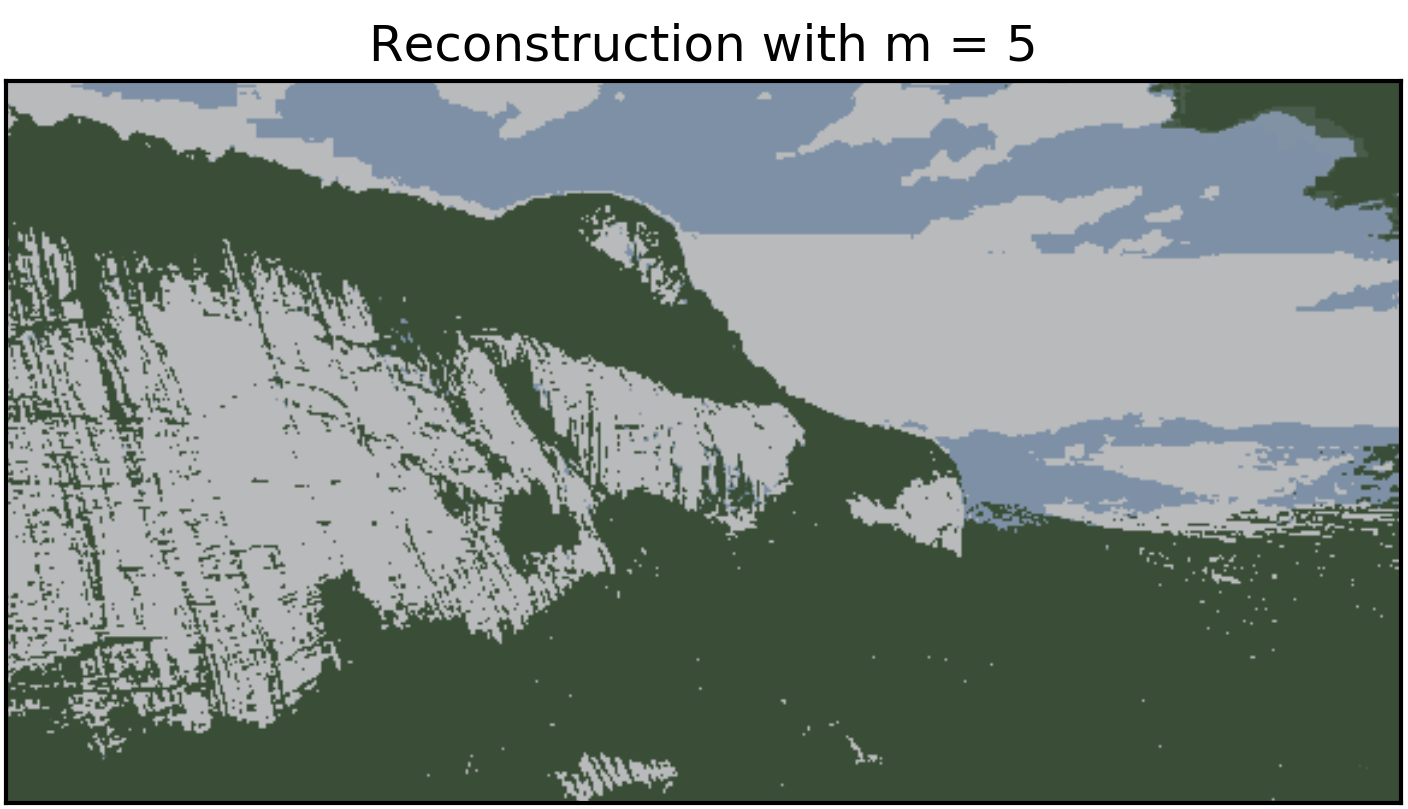
\includegraphics[width=0.6\textwidth]{./figures/self_tf_5.png}
\caption{\label{fig:self_tf_5} Mountain with 5 Gaussian Mixtures}
\end{figure}

\begin{figure}[H]
\centering
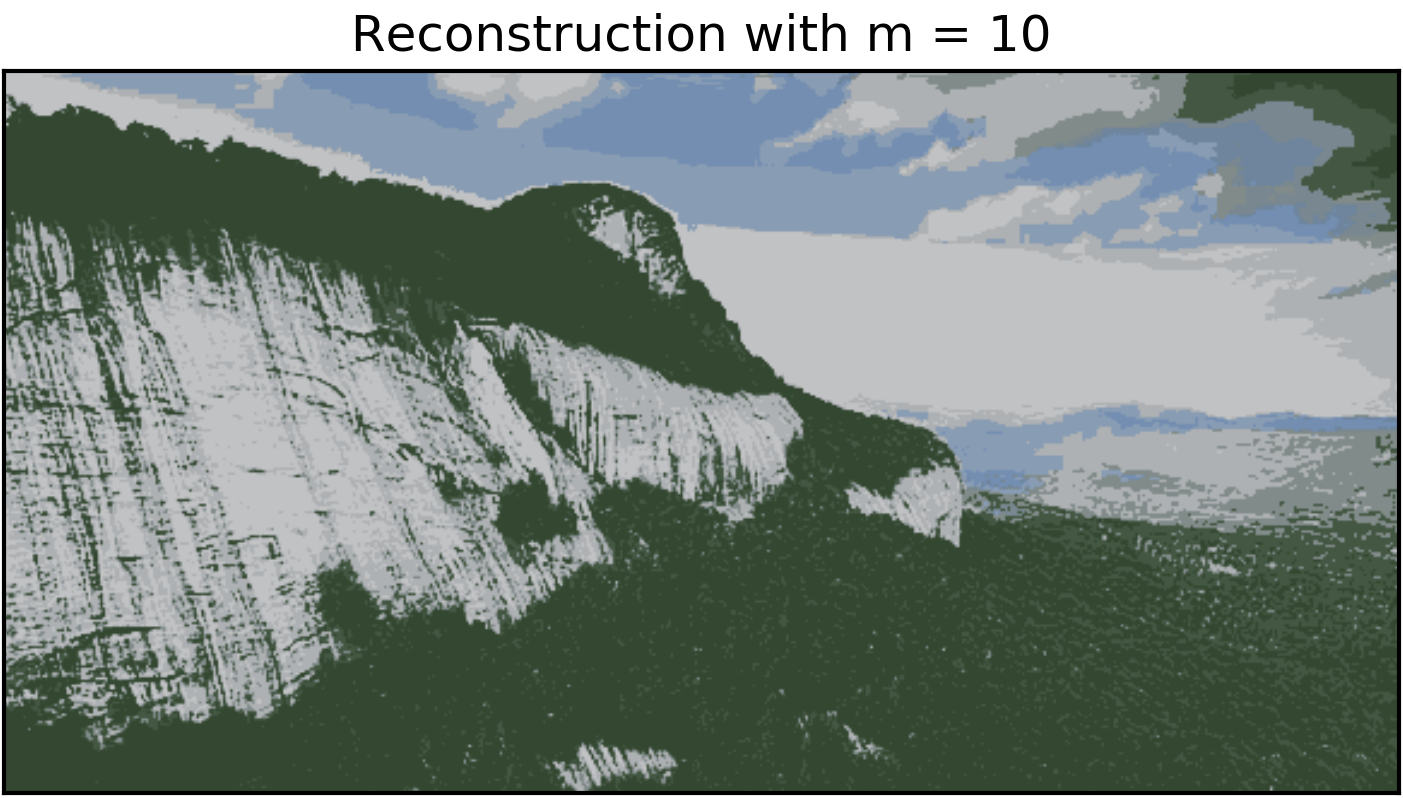
\includegraphics[width=0.6\textwidth]{./figures/self_tf_10.png}
\caption{\label{fig:self_tf_10} Mountain with 10 Gaussian Mixtures}
\end{figure}

\noindent Compare the result from self-code and TensorFlow, we may conclude that, for self-written code, it is easy to reach some local maximum and some good initialization should be implemented in the future.

\clearpage
\end{document}

